\section{Methods}
\label{sec:methods}

\subsection{The CoRR Studies have disparate demographic characteristics}
\label{sec:demo}
% refer back to description of CoRR in non-novel methods
The motivation for our development of a modified framework for defining, detecting, and harmonizing for batch effects is the neuroimaging mega-study produced by the Consortium for Reliability and Reproducibility \cite{corr}, a collection of over $3$,$600$ functional neuroimaging measurements from over $1$,$700$ individuals spanning $27$ separate datasets. Figure \ref{fig:demographic}A  explores the demographic characteristics for the individuals in the CoRR mega-study. Many of the studies have a narrow age range, and several studies only include females. Because sex \cite{Weis2020Mar,Ingalhalikar2014Jan,Satterthwaite2015Sep}, age \cite{Varangis2019,Sala-Llonch2015,Hampson2012Sep}, and continent \cite{Misiura2020,JianqiaoGe2023Jan} are variables that have been associated with brain connectivity, they serve as demographic covariates used in our investigation.

\begin{figure}[!h]
    \centering
    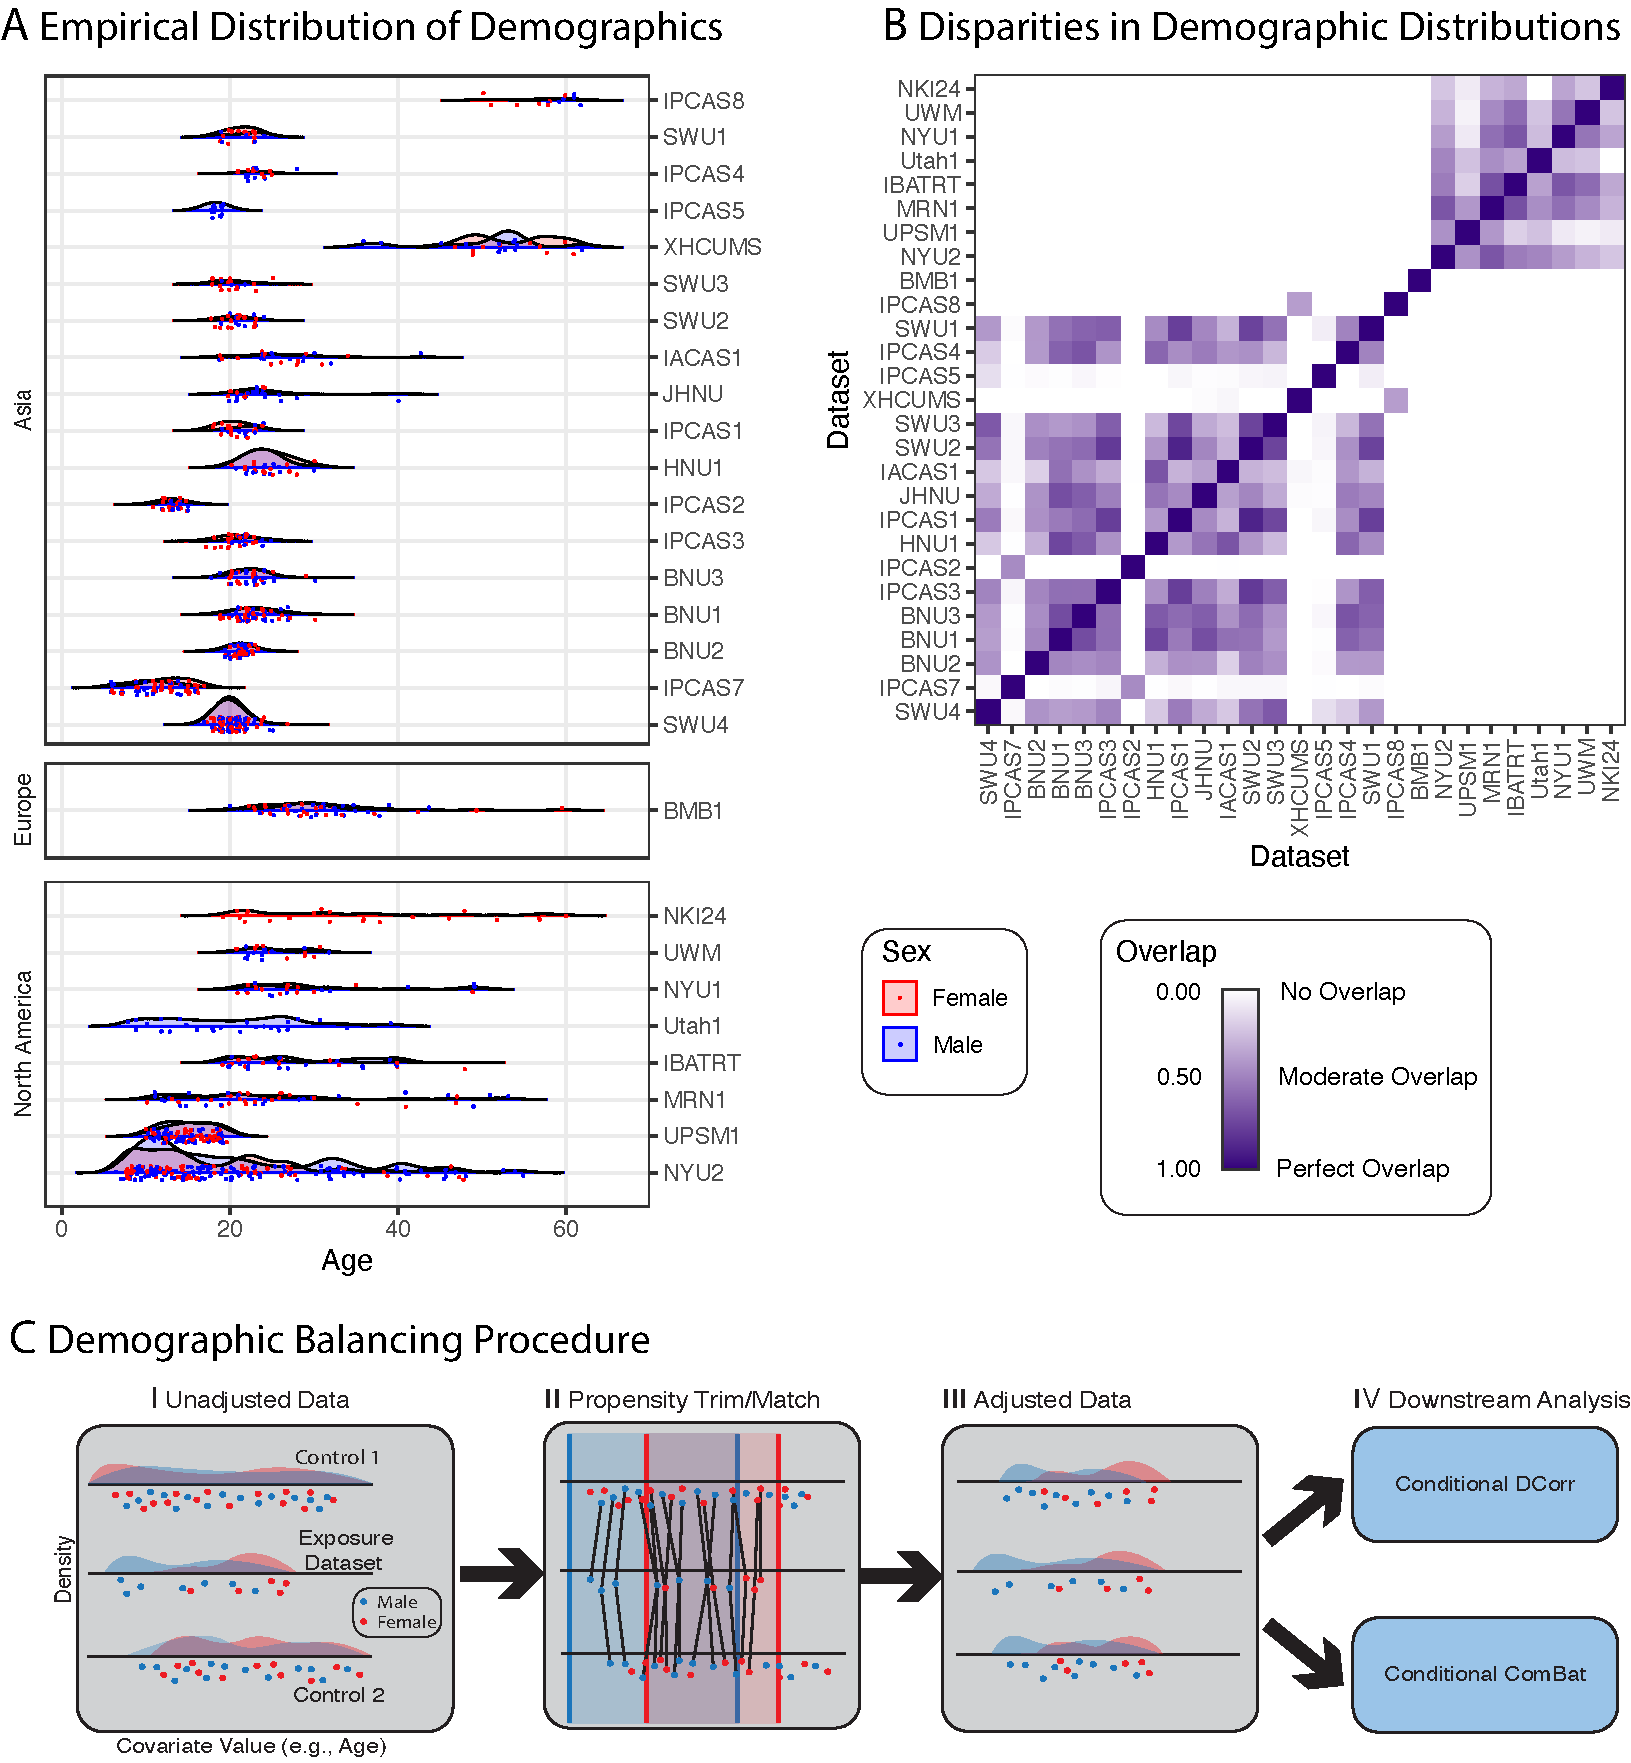
\includegraphics[width=\linewidth]{Figures/Content/demographic.pdf}
    \caption{\textbf{Demographic data for each of the $N=27$ studies from the CoRR Mega-Study}. \textbf{(A)}  Each point represents the age of a participant corresponding to a single measurement, rows are studies, boxes are continents, and color indicates sex. 
    % Empirical density is estimated across individuals corresponding to each sex within each study, where height is scaled by the number of measurements for each $(\textrm{sex}, \textrm{study})$ pair. 
    \textcolor{black}{\textbf{(B)} Even with only $3$ covariates made available (sex, age, continent of measurement) the CoRR studies generally show extremely poor covariate overlap \cite{Pastore2019}. This makes inference regarding batch effects difficult. \textbf{(C)} The demographic balancing procedure, to demographically align poorly balanced datasets using Causal \Dcorr~or \cccombat. (C.I) The unadjusted datasets are imbalanced in covariate distributions. The smallest dataset, the \textit{reference}, has a narrower age distribution than the controls. (C.II) Propensity trimming (shaded boxes) and matching (lines) are conducted to identify reasonable matches between the reference and the control datasets. (C.III) The adjusted datasets have far improved demographic overlap after propensity trimming, matching, and removing reference subjects who do not have suitable matches in the control datasets. (C.IV) Downstream batch effect detection via \Dcorr~or correction using \Combat~are performed on the data using conditional strategies on the adjusted data.}}
    \label{fig:demographic}
\end{figure}

\textcolor{black}{Figure \ref{fig:demographic}B investigates the level of demographic overlap in the CoRR mega-study, using the distribution-free overlapping index \cite{Pastore2019}, as discussed in Appendix \ref{app:overlap}. Many of the datasets do not overlap at all, making inference about batch effects (e.g., via detection or harmonization) impossible without making major assumptions. This is particularly troublesome, as the covariate records for the CoRR mega-study common to all sites include only three covariates: age, sex, and continent of measurement. The addition of successive covariates can only reduce the estimated overlap between the pairs of datasets, so having poor overlap on such a coarse set of covariates indicates that the actual demographic overlap may be even lower.}

\subsection{Defining batch effects}

{\edits{For a formal description of the below definitions, see \citet{Bridgeford2023Jul}. 

Informally, we adopt the following notation to describe batch effect correction. We assume that $Y$ represents an observed measurement of interest (e.g., a connectome), $T$ represents the batch in which the measurement is collected, $X$ represents covariates which are measured associated with the individual for whom the measurement was collected (e.g., age or biological sex), and $Z$ represents covariates which are not measured associated with the individual for whom the measurement was collected. The quantity $Y(t)$ represents the measurement that would have been observed, had the measurement been collected in a given batch $t$. The key distinction is that $Y$ represents the \textit{actual} measurement, which is collected and studied. On the other hand, $Y(t)$ is a hypothetical measurement, which is only actually observed for the case where $T = t$ in most experimental contexts \cite{Cole2009Jan}. That is, individuals have a potential measurement $Y(t)$ for every possible batch, but only a single of these potential measurements are studied under standard observational contexts. That the observed measurements $Y$ given the batch (or measured covariates) and the potential measurements $Y(t)$ do not, in general, have similar distributions is known as the ``fundamental problem of causal inference.'' This problem requires resorting to additional assumptions to make conclusions on the basis of the observed data.

Using this convention, a batch effect is defined in Definition \ref{def:causal_batch_informal}.

\begin{definition}[Causal Batch Effect]
A causal batch effect exists between two batches $t$ and $t'$ if $Y(t)$ and $Y(t')$ have different distributions.
\label{def:causal_batch_informal}
\end{definition}

In light of this definition, a batch effect can be conceptualized as the \textit{potential} measurements having different distributions between a given pair of batches. A batch effect is present if an individual's measurements differ if they \textit{would have been measured} in batches $t$ and $t'$. We can similarly define batch effect correction to be a function of the potential measurements and the batch which remove this disparity, in Definition \ref{def:batch_correct_informal}.

\begin{definition}[Batch Effect Correction]
A function $g$ corrects a batch effect between $Y(t)$ and $Y(t')$ if $g(Y(t), t)$ and $g(Y(t'), t')$ have the same distribution.
\label{def:batch_correct_informal}
\end{definition}

In this case, a function corrects a batch effect if the \textit{potential} measurements have the same distribution after application of the function $g$. Estimation of this function $g$ from the observed data (which, often, does not include realizations of every \textit{potential} measurement for each individual) therefore presents the hurdle of batch effect correction. The major conceptual leap in the aforementioned definitions is that, under standard contexts, these statements are about \textit{potential} measurements rather than \textit{realized} measurements. In other words, causal claims regarding potential outcomes are only valid on the basis of the observed data insofar as the reasonableness of the assumptions upon which they rest.

\subsubsection{Associational Effects}

In an associational context, we observe measurements $y_i$ and batches $t_i$ for each individual $i \in [n]$, so effects can only be determined from $Y$ and $T$. 

\begin{flushleft}\begin{definition}[Associational Effect]
% Suppose the setup described above. 
An associational effect exists between batches $t$ and $t'$ if $Y | T = t$ and $Y | T = t'$ have different distributions.
\label{def:ass_site_effect_informal}
\end{definition}
\end{flushleft}

Similarly, associational effect correction estimates the function $g$ using only the observed measurements and the batches. Under standard contexts, associational effects will often poorly characterize whether a batch effect is present. Consider, for instance, if in one batch $t$, we tend to measure older individuals, whereas in another batch $t'$, we tend to measure younger individuals. If age is related to the measurement we obtained, then the differences between $Y | T = t$ and $Y | T = t'$ could be due to age or batch identity, and we have no way of differentiating whether the effect is a \textit{bona fide} batch effect versus merely an associational effect. A sufficient condition for an associational effect to facilitate detecting or estimating a batch effect would be that individuals are randomized to each batch, in that individuals are assigned to be measured in particular batches \textit{pre-hoc}. Associational effect detection can be facilitated via \Dcorr~\cite{Szekely2007Dec} and associational effect correction can be facilitated via \Combat~\cite{Johnson2007Jan}.

\subsubsection{Conditional Effects}

In a conditional context, we observe measurements $y_i$, batches $t_i$, and covariates $x_i$ for all individuals $i \in [n]$, so effects can be determined from $Y$, $T$, and $X$.

\begin{flushleft}\begin{definition}[Conditional Effect]
A conditional effect exists between batches $t$ and $t'$ if for some covariate $x$, $Y | T = t, X = x$ and $Y | T = t', X = x$ have different distributions.
\label{def:ass_site_effect_informal}
\end{definition}
\end{flushleft}

Conditional effect correction estimates the function $g$ using the observed measurements, the batches, and the covariates. Conceptually, a conditional effect is equivalent to a batch effect if two conditions hold:
\begin{enumerate}[leftmargin=*]
    \item  the measured covariates overlap in distribution between the batches (propensity overlap), and
    \item given the measured covariates, we can ignore how people ended up in one batch versus the other.
\end{enumerate}

The former condition denotes that both batches must contain similar groups of people (in terms of measured covariates), and the latter condition specifies that the measured covariates $X$ tell us all of the information needed to ``exchange'' measurements from one batch to the other. Borrowing the preceding example, even if we observe more young people in a batch $t$, that we still observe \textit{some} young people in the other batch $t'$. In this sense, the measured covariates contain the information needed to ``deconfound'' disparities that might be batch effects or veridical effects due to upstream covariates. Therefore, when we make subsequent comparisons, we do not need to guess what people with similar covariates would have looked like in the other batch, and vice versa.

In this fashion, our comparisons can be thought of as locally (with respect to the covariates) exchanging a realized measurement $Y$ in batch $t$ with a realized measurement $Y$ in batch $t'$, where both individuals have similar covariates $x$. Intuitively, these comparisons can therefore be conceptualized as synthetically comparing $Y(t)$ and $Y(t')$ (the target estimand for establishing a batch effect) by using observed measurements $Y$ from individuals who are similar on the basis of the covariates $X$ between the two batches. The former condition ensures that we can make this intuitive step over the entire span of covariates in our batches. Conditional effect detection can be facilitated via \cdcorr~\cite{Wang2015}, and conditional effect correction can be facilitated via \ccombat~\cite{Johnson2007Jan}.

In practice, we never know whether the propensity distributions overlap; we can only estimate them from the data. If our estimated propensities do not overlap given finite data, we again cannot reasonably differentiate between differences in the two groups being due to \textit{bona fide} batch effects or empirical differences in the propensity distributions. This motivates a third approach. 

\subsubsection{Adjusted Effects}

As before, we observe measurements $y_i$, batches $t_i$, and covariates $x_i$ for all individuals $i \in [n]$, and we determine effects from $Y$, $T$, and $X$. Prior to assessing the equality of any distributions, however, we weight the observations such that the observed covariate distributions are rendered approximately overlapping.

\begin{flushleft}\begin{definition}[Adjusted Effect]
An adjusted effect exists between batches $t$ and $t'$ if after re-weighting samples such that $X | T = t$ and $X | T = t'$ are approximately overlapping (or, alternatively, approximately equal), $Y | T = t, X = x$ and $Y | T = t', X = x$ have different distributions.
\label{def:ass_site_effect_informal}
\end{definition}
\end{flushleft}

Adjusted effect correction amounts to estimating the function $g$ using the observed measurements, the batches, and the covariates, but placing higher priority on up-weighted samples and lower priority on down-weighted samples in the estimation process depending on whether they are sufficiently represented in both batches of interest. Adjusted effects, by default, satisfy the first criterion for a conditional effect to be a batch effect. This is because rendering measured covariate distributions approximately equal intuitively is a more strict criterion than simply ensuring that they approximately overlap. The reason that we believe that re-weighting to ensure approximate covariate distribution equality is desirable for effect correction, versus simply approximate covariate overlap, is discussed in Section \ref{sec:results:sims} and Appendix \ref{app:sim_batch_adj}. Adjusted effect detection can be facilitated via \ccdcorr~\cite{Bridgeford2023Jul}, and adjusted effect correction can be facilitated with \cccombat~(described in Section \ref{sec:cccombat}).

We still must satisfy the latter criterion for a conditional effect to be a batch effect; that is, given the measured covariates, we can ignore how people ended up in one batch versus the other. This assumption has the same interpretation as before.

\subsubsection{Crossover Effects}

We observe measurements $y_i(t)$ and covariates $x_i(t)$, for all individuals $i \in [n]$ and for all batches $t \in [T]$. In this case, we can make statements on the basis of $Y(t)$, and may not need to resort to local exchangeability (similar individuals across batches) as before. \textit{Crossover effects in general require the fewest assumptions to derive causal conclusions, since we directly observe all possible potential measurements for each individual}.

\begin{flushleft}\begin{definition}[Crossover Effect]
A crossover effect exists between batches $t$ and $t'$ if, given that $\left(X(t), Z(t)\right)$ and $\left(X(t'), Z(t')\right)$ are sufficiently similar, $Y(t)$ and $Y(t')$ have the same distribution.
\label{def:ass_site_effect_informal}
\end{definition}
\end{flushleft}

We are certain that any \textit{traits} of the participants (i.e., variables that are constant for a given participant, such as genome) are the same across the two groups since the group members are identical (even if we did not measure these traits). However, \textit{states} may differ as they may be functions of location or time. For example, if being measured impacts subsequent states, then a crossover effect may not be indicative of a causal batch effect without further assumptions and/or experimental design considerations (such as randomizing exposure order across participants, or resorting to adjusted effect strategies as before if these states are measured). 

In the case where participant states are unchanging or are randomized, we can resort directly to associational strategies for subsequent detection or removal, and can make causal conclusions about batch effects with few additional considerations. In the case where participant states are changing and are not randomized but are measured, we can resort to adjusted strategies for adjusted effect detection or removal. For the latter, we need to make the same assumptions as before; that is, that given the measured covariates (which include the changing states), we can ignore how people ended up in one batch versus the other.}}

\subsection{Detecting and mitigating causal batch effects}
\label{sec:cccombat}
At present, literature approaches for detecting and mitigating batch effects tend to focus attention heavily on effects which could be classified as associational or conditional, which for the above listed reasons, fail to adequately account for confounding biases. To this end, we propose a simple technique to augment associational and conditional strategies and derive stronger causal claims. We propose the following strategy:
\begin{enumerate}[leftmargin=*]
    \item Use classical causal procedures to re-weight the measurements from the batches so that the demographic distributions across all batches to be considered overlapping or are approximately equal. For rendering the covariate distributions approximately overlapping, we leverage vector matching \cite{Lopez2014}. For rendering the covariate distributions approximately equal, we leverage propensity trimming followed by nearest neighbor matching \cite{Stuart2010Feb,Powell2020Sep}. 
    \item Apply classical procedures for detection or removal of {\edits{conditional}} effects. For the purposes of elucidating the benefits of this perspective, we choose to apply our techniques to \cDcorr~for batch effect detection \cite{Wang2015,Bridgeford2023Jul}, and \ccombat~for batch effect removal \cite{Pearl2010Jul,Johnson2007Jan,Leek2010-ua,Leek2015-jc,Wachinger2020Feb,Yu2018Nov,Pomponio2020Mar}.
\end{enumerate}

For a more technical description of the causal procedures employed in this manuscript, see Appendix \ref{app:causal_procedures}. It is important to note that we do \textit{not} make the claim that the specific choices for re-weighting measurements (propensity trimming followed by nearest-neighbor matching) are necessarily the best possible approach to balancing the demographic distributions across the batches. Indeed, there are almost two decades of research dedicated towards making these design choices for observational studies. Rather, we chose simple, principled, and straightforward approaches for illustrative purposes. Our simulations contained herein and in our related manuscript \cite{Bridgeford2023Jul} elucidate that even these possibly simplistic balancing approaches are sufficient to highlight substantial shortcomings in the existing literature for batch effects and causal effect testing, as well as the substantial benefits of a causal perspective.

\subsection{Batch effects in biological datasets}

\begin{figure}[!h]
    \centering 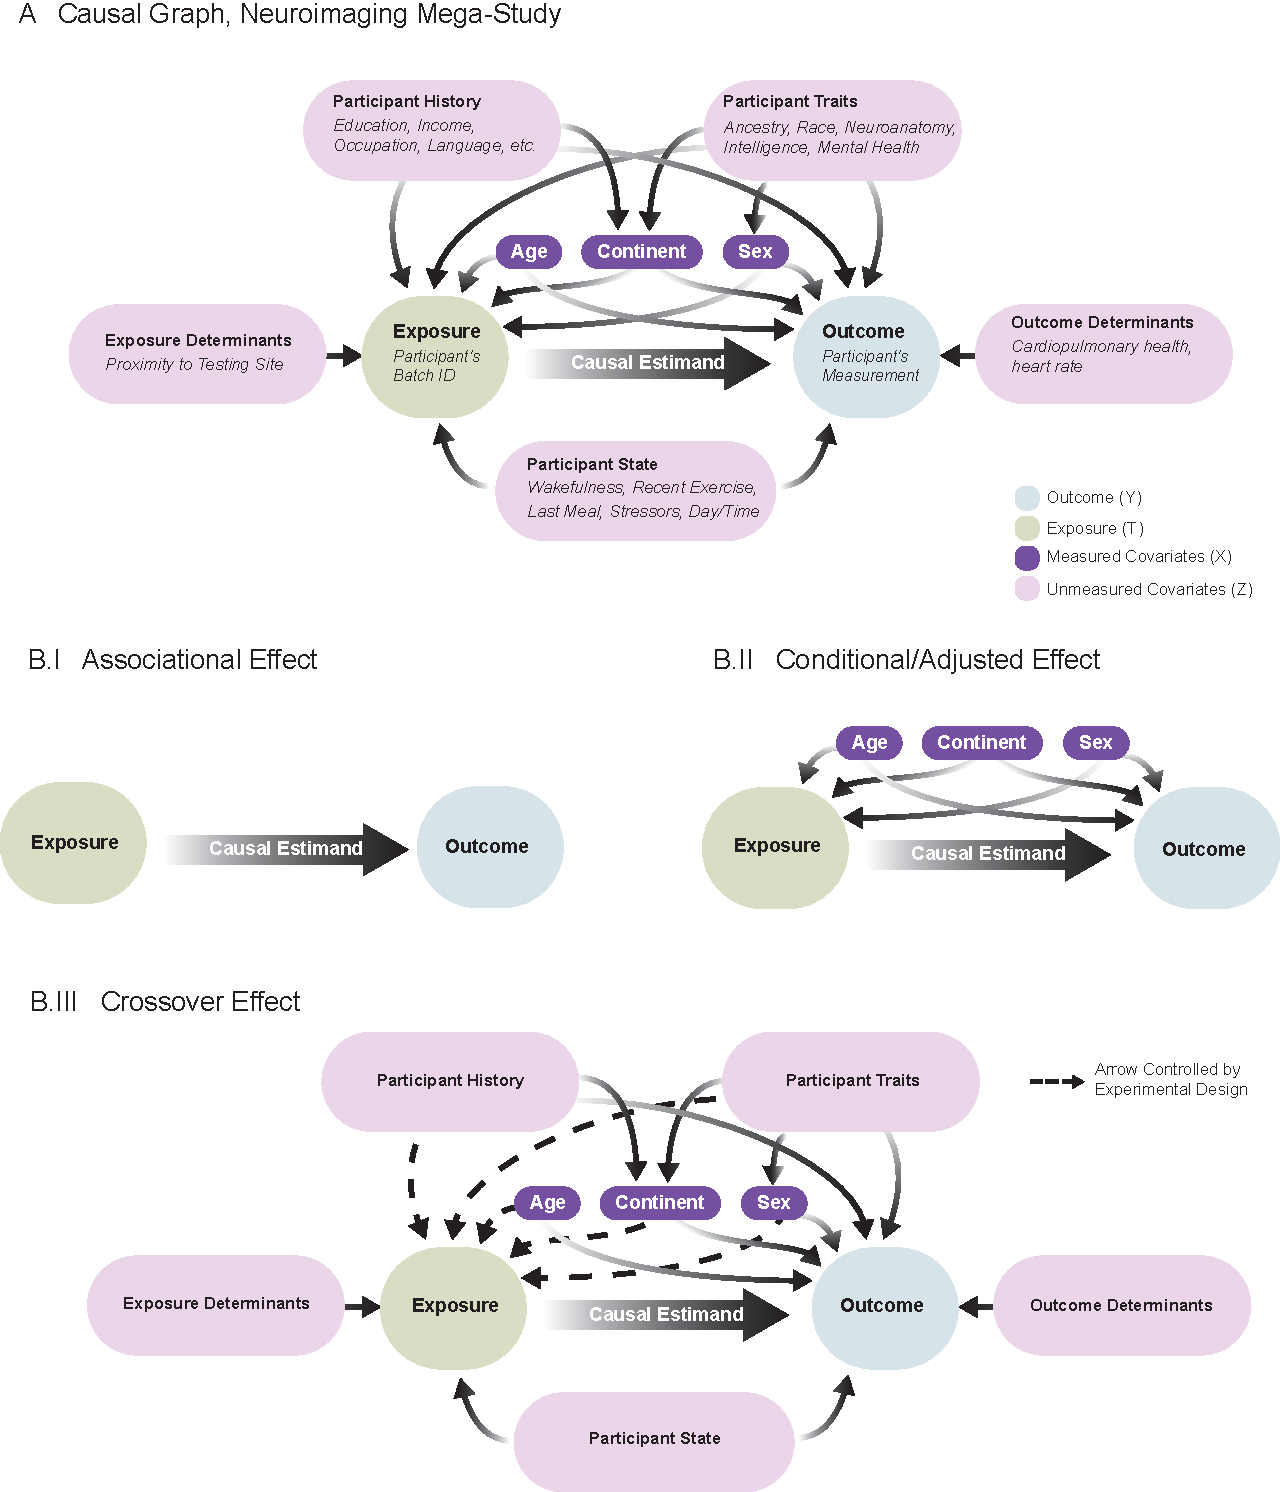
\includegraphics[width=\linewidth]{Figures/Content/CoRR_dag.pdf}
    \caption{\textbf{Causal Graph of Study Covariates}. \textbf{(A)} A causal directed acyclic graph (DAG) illustrating potential relationships which can reasonably be assumed to underlie a mega-study. Descriptions reflect possible attributes that might fall into the specific exposures, outcomes, and covariates for a neuroimaging study, for illustration purposes. \textbf{(B)} DAGs which illustrate the assumptions which underlie assorted effects in order for those effects to be causal. Associational effects \textbf{(B.I)} are causal when all external covariates are independent the exposure and outcome. Conditional effects and adjusted effects \textbf{(B.II)} are causal when the strong ignorability condition holds, and in particular when the measured covariates close backdoor paths. Crossover Effects \textbf{(B.III)} are causal when participant states are non-confounding between the exposure and the outcome. The experimental design of a crossover study ensures that other forms of measured and unmeasured covariates are non-confounding.}
    \label{fig:dag}
\end{figure}
The four effects discussed above have immediate practical implications on measuring batch effects in modern biological datasets. To this end, we demonstrate the applicability of these effect types in the context of a the CoRR mega-study, in which measurements are collected from individuals across various batches (the \textit{exposures}). The logical process, however, extends beyond this context to many other biological data modalities, such as genomics. Figure \ref{fig:dag}A shows a directed causal graph which underlies a typical mega-study. Directionality of arrows (e.g., $X \rightarrow Y$) indicates that the factor $X$ can influence the variable $Y$. For instance, aging may cause changes to the brain, which are reflected in the measurements. The exposure is the batch in which participants' data are collected, and the outcomes are the measurements themselves. We seek to estimate the \textit{causal estimand}, which is the causal effect of the exposure to a particular batch on the outcome (the \textit{measurement}). Numerous covariates, both known and unknown, impart potentially confounding biases, in which the variables can influence both the exposure and the outcome. For instance, one batch collected in a children's hospital may tend to over-sample younger individuals relative to other batches, and younger children may have distinct patterns of brain connectivity compared to older children. {\edits{For this investigation, we use age and sex (which are commonly used for adjusting for batch effects) as well as continent as measured covariates in subsequent analyses. We depart from many previous harmonized analyses by leveraging continent due to the growing literature \cite{JianqiaoGe2023Jan,Park2010Jul} which suggest differences in brain function for individuals across cultures. Unaccounted confounding via culture/race (for which continent serves an imperfect surrogate) may yield confounding biases in subsequent analysis, in which batch effects may be conflated with veridical demographic differences.}} 

Unmeasured covariates are often prominent confounders in biological datasets, making proper causal analyses troublesome. \textit{Participant history} involves variables related to specific life experiences, both environmental and societal, that the individual has been exposed to. \textit{Participant traits} are characteristics of a person that remain relatively constant over time. \textit{Participant states} refer to characteristics of a person that change over an individual's lifetime. \textit{Exposure determinants} are factors which impact batch membership for a particular individual, but do not impact the measurement itself. \textit{Outcome determinants} are factors which do not impact the batch assignment, but impact the outcome. In this particular study, people are not explicitly recruited on the basis of traits or histories which may affected by their measurements (e.g., neurodiversities). This yields that the causal graph is also acyclic, or a DAG. A discussion on what happens in the event that the causal graph is not a DAG is provided in Section \ref{sec:discussion}.

Figure \ref{fig:dag}B illustrates the implicit DAGs that are sufficient such that if they characterized the data, then each of the four effect types discussed above become valid causal batch effect estimands. 
If no covariates exist (observed or unobserved), then an associational effect is a causal effect (Figure \ref{fig:dag}B.I). 
% TODO re-read below
% While conditional and associational effects can be causal in the presence of confounding when confounding variables are measured, neither effect is causal when confounding variables are unmeasured (Figure \ref{fig:dag}B.II).
Crossover effects can account for many types of measured and unmeasured covariates which are confounding (Figure \ref{fig:dag}B.III). Because of the crossover property, the batches will be balanced across certain measured and unmeasured covariates, specifically patient history and traits. Hence, many of the confounding variables from Figure \ref{fig:dag}A are deconfounded. However, unmeasured changes in participant state between different exposure groups (such as measuring individuals only during the daytime in one batch and only during the night time in another batch) remain potential confounders if not carefully balanced across exposure groups through either randomization or direct experimental intervention. 
